\documentclass[journal]{IEEEtran}

\usepackage{graphicx}
\usepackage{listings}
\usepackage{color}
\definecolor{codeColor}{rgb}{0.4, 0.6, 0.8}
\lstset{keywordstyle=\color{codeColor},language=Octave,stepnumber=1,basicstyle=\footnotesize}

\usepackage{enumitem}

\newenvironment{steps}[1]{\begin{enumerate}[label=#1 \arabic*]}{\end{enumerate}}

\makeatletter
\def\step{
   \@ifnextchar[ \@step{\@noitemargtrue\@step[\@itemlabel]}}
\def\@step[#1]{\item[#1]\mbox{}\\\hspace*{\dimexpr-\labelwidth-\labelsep}}
\makeatother

\begin{document}

\title{ Solucion de Ecuaciones No Lineales}
\author{Rub�n Cuadra A01019102}

\maketitle
\begin{abstract}
	Manual de usuario:  'noLineal.m', el objetivo de este documento es documentar la implementacion del metodo Newton-Raphson y metodo de Secante como metodos numericos
\end{abstract}

\section{Introduccion}
	El codigo consiste en un archivo llamado de la misma manera que la funcion el cual recibe 4 argumentos y nos regresa 3 respuestas
\lstinputlisting[ firstline=1, lastline=1]{noLineal.m}

	\textbf{x0}  puede ser un arreglo de 2 posiciones o 1 numero. Esto depende de acuerdo al \textbf{metodo} que usemos, donde True(1) es Secante y False(0) es Newton-Raphson
	
	\textbf{eps} se refiere a un numero, por lo general decimal, que sirve como criterio de convergencia, nos indica el rango que tiene el metodo para llegar a la solucion 
	
	\textbf{maxIt} es un numero entero que definira el numero de iteraciones en las que se debe obtener el resultado, en caso de que el codigo no llegue a la solucion basado en el eps nos devolvera un error
\section{Comprension del algoritmo}
	
\subsection{Newton-Raphson}
Se busca llevar la ecuacion $f(x) =0$ a la forma $x = g(x)$ para que$g'( \bar{x} ) =0$

Entonces, en la funcion pasamos un valor inicial de X, un criterio de convergencia EPS y el numero de iteraciones maximas para llegar a la solucion, esto debido a la probabilidad de oscilar asi como de diverger. La formula usada es: \begin{equation} x = x^{}_0-\frac {F(x^{}_0)}{F'(x^{}_0)} \end{equation}
\begin{steps}{Paso}
\step Inicializar valores a regresar con datos de Error
\step Iniciar ciclo en iter=0 hasta que iter=maxiters
\step Aplicar formula 1 en una variable designada temp
\step Comparar temp-$x^{}_0$ Si es menor al criterio de convergencia, regresar exito y temp como respuesta
\step Si llegamos aqui convertir $x^{}_0$ en temp y repetir paso 3, sumando 1 al iterador
\step Regresar valores de error si se acabaron las iteraciones
\end{steps}
\subsection{Secante}

En el metodo de secante obtenemos 2 valores $x^{}_0$  y $x^{}_1$ asi como un EPS y de igual manera el numero maximo de iteraciones, con esto calculamos el proximo punto. Usamos la formula:
\begin{equation}x_{n+1} = x_n - \frac{x_n-x_{n-1}}{f(x_n)-f(x_{n-1})} f(x_n)  \end{equation}
\begin{figure}
    \centering
    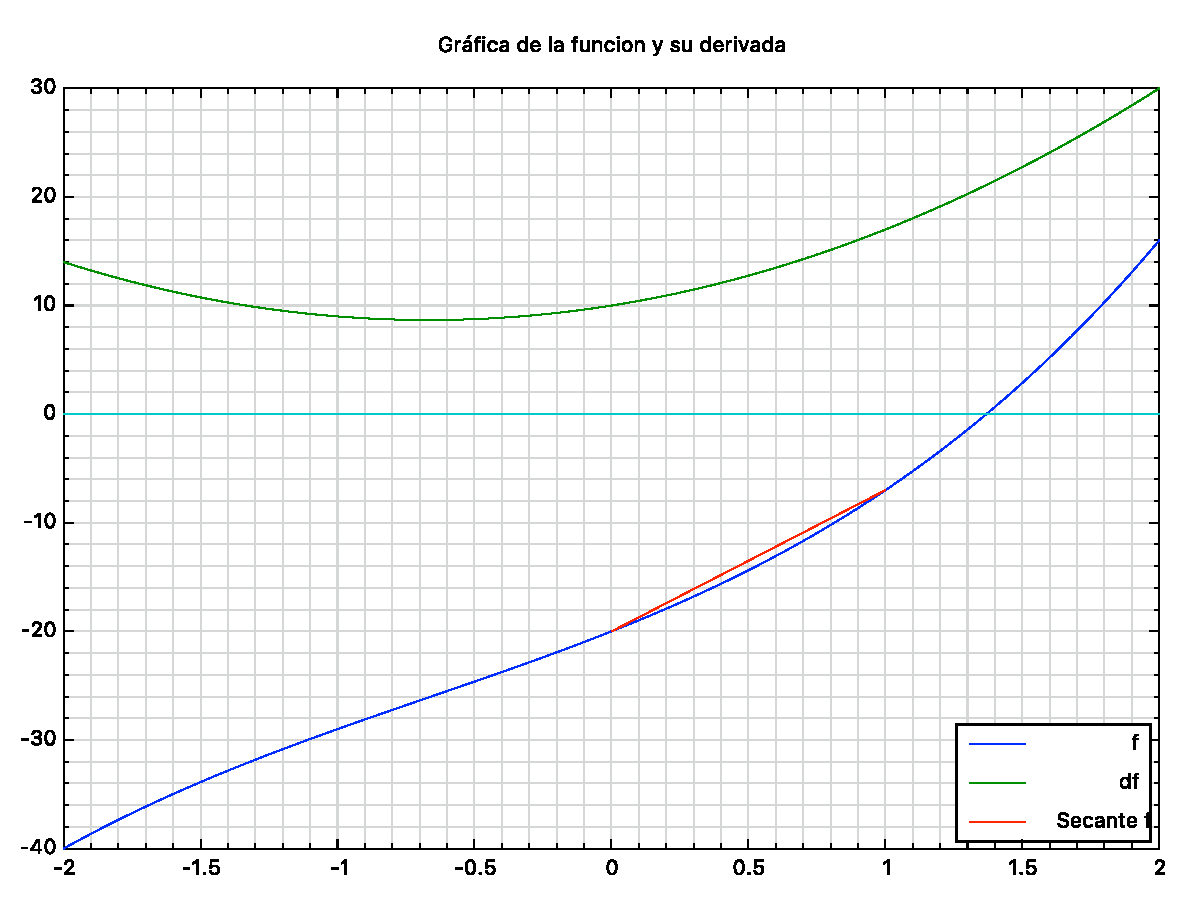
\includegraphics[width=3.50in]{d_df}
    \caption{Ecuaciones de f.m y df.m respectivamente, la secante se encuentra desde x0=0 a x1=1}
    \label{examplefigure}
    Archivos .m respectivamente
    \lstinputlisting[language=Octave]{f.m}
   \lstinputlisting[language=Octave]{df.m}
\end{figure}

\begin{steps}{Paso}
\step Inicializar valores a regresar con datos de Error
\step Iniciar ciclo en iter=0 hasta que iter=maxiters
\step Aplicar formula 1 en una variable designada next
\step Comparar next-$x^{}_1$ Si es menor al criterio de convergencia, regresar exito y next como respuesta
\step Si llegamos aqui convertir $x^{}_0=x^{}_1$ y $x^{}_1= next$ en temp y repetir paso 3, sumando 1 al iterador
\step Regresar valores de error si se acabaron las iteraciones
\end{steps}

\section{Ejemplo}
Mandamos a llamar la funcion desde un archivo main.m.
Asi mandamos a llamar la funcion con metodo secante si queremos usar de valores x iniciales 0 y 1, queriendo un EPS de 0.001 y un maximo numero de iteraciones de 10
\lstinputlisting[language=Octave,firstline=1,lastline=1]{main.m}
El resultado seria:
\lstinputlisting[language=Octave,firstline=2,lastline=4]{main.m}
Si ahora queremos mandar a llamar la funcion con el metodo Newton-Raphson la llamariamos con los mismos valores pero la x inicial basta con ser un numero, en este caso 1
\lstinputlisting[language=Octave,firstline=5,lastline=5]{main.m}
y nos devolveria
\lstinputlisting[language=Octave,firstline=6,lastline=9]{main.m}

Donde en ambos casos Error=0 significa que NO hay error. i = 2 | i = 3 nos define el numero de iteraciones respectivamente. x es la solucion


\section{Conclusion}
No todos los metodos numericos son perfectos, las funciones pueden oscilar o diverger, ya que ambos son de segundo grado son bastante rapidos pero claro, Newton suele llegar mas rapido si logramos obtener la derivada de la funcion, que suele llevar mas procesador.
\footnotetext{Los acentos no se pudieron agregar por cuestion de la codificacion}
\end{document}
